\documentclass[lecture.tex]{subfiles}

\begin{document}

\exercice{}
%\video{https://youtu.be/blablabla}
\enonce{rdm-0002}{Poutre Encastrée-libre 2D}

\begin{center}
  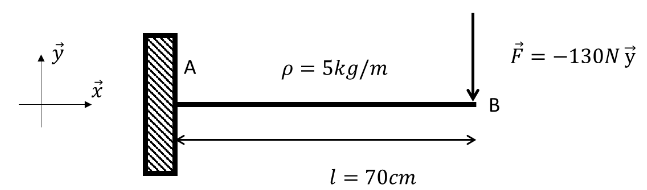
\includegraphics[scale=0.4]{exo-poutre2d.png}
\end{center}

\begin{enumerate}
  \item Faire le bilan des actions mécaniques extérieures à la poutre.
  \item Déterminer le degré d’hyperstatisme de la poutre.
  \item Trouver les inconnus de liaison de la structure (les efforts et les moments résultants de l’encastrement).
  \item Conclure sur l’effet du poids.
\end{enumerate}

\finenonce{rdm-0002}
\finexercice


\end{document}
